\section{Evaluation}
\label{sec:evaluation}

Our \tern implementation consists of 8,934 lines of C++ code, including 827
lines for the instrumentor implemented as an LLVM pass; 5,451 lines for
the proxy, schedule cache, memoizer, and replayer; and 2,656 lines for
modifications to \klee.

We evaluated \tern on a diverse set of 14 programs, ranging from two server
programs, Apache and MySQL, to one parallel compression utility, \pbzip, to
11 scientific programs in \splash.\footnote{The version of the
  SPLASH2~\cite{lu:bugbench} we acquired has 12 programs, one of which does
  not compile on our evaluation machine.}
%  \pbzip and \splash programs are batch programs.
% Table~\ref{table:apps} column Size shows the size of these programs.  

Our main evaluation machine is a 2.66 GHz quad-core Intel machine with 4
GB memory running Linux 2.6.24.  When evaluating \tern on server programs, we
ran the server on this machine and the client on another to avoid
unnecessary contention.  These machines are connected via 1Gbps LAN.  We
compiled all programs down to machine code using \v{llvm-gcc -O2} and
LLVM's bitcode compiler \v{llc}.

We focused our evaluation on four key questions:
\begin{enumerate}

\item Is \tern easy to use (\S\ref{sec:ease-of-use})?

\item Does \tern make multithreaded programs stable across different inputs
  (\S\ref{sec:stability})?

\item Does \tern incur high overhead (\S\ref{sec:overhead})?

\item Does \tern make multithreaded programs deterministic on the same
  input (\S\ref{sec:determinism})?

\end{enumerate}




%% \begin{table}
%% \centering
%% \small
%% \begin{tabular}{ll}
%% {\bf Program} & {\bf Synthetic} & {\bf Real} \\
%% \hline
%% Apache & ApacheBench  &  CS web trace, Wikipedia trace \\
%% MySQL  & DBT2~\cite{dbt2}& Wipipedia trace \\   
%% \pbzip & Compressing files with various sizes \\   
%% \end{tabular}
%% \caption{\em Programs evaluated.}
%% \end{table}

%% We evaluated \tern on a diverse set of 14 programs, ranging from two server
%% programs Apache and MySQL, to one parallel (de)compressing utility \pbzip,
%% to 11 scientific programs in \splash (all programs
%% from~\cite{lu:bugbench}, except one that did not compile).  \pbzip and
%% \splash programs are batch programs.
%% % Table~\ref{table:apps} column Size shows the size of these programs.  

%% We used the following workloads in our experiments.  For MySQL, we chose
%% SysBench~\cite{sysbench} with both simple and advanced transaction workload. 
%% The simple workload randomly selects database records, and the advanced transaction workload randomly
%% selects, updates, deletes, and inserts records.  We made both SysBench and ApacheBench CPU bound by fitting
%% the database or web contents within memory; we also ran both the benchmark client
%% and the server on different machines in order to avoid hardware contention, and we 
%% carefully chose workload to make sure network bandwidth was not the bottleneck.  
%% % Unless otherwise specified, we run 16 worker threads for MySQL and
%% % Apache because they perform the best in this setting; we run four worker
%% % threads for \pbzip and \splash applications because they are
%% % CPU-intensive and our evaluation machine has four cores.

%% We used two evaluation machines: a 2.66 GHz single-CPU quad-core Intel
%% machine with 4 GB memory and 32-bit Linux 2.6.24 and a 1.9 GHZ 4-CPU
%% 12-core AMD machine with 64 GB memory and 64-bit Linux 2.6.24. We
%% compiled programs down to machine instructions using \v{llvm-gcc -O2}
%% and LLVM's bitcode compiler.  We measured overall execution time for
%% batch programs and throughput (short as TPUT) and response time (short
%% as RESP) for server programs.  We reported \tern's nomalized overhead,
%% the smaller the better.  For all the performance numbers reported, we
%% repeated the experiment 100 times and took an average.

\subsection{Ease of Use}\label{sec:ease-of-use}

\begin{table}
\centering
\footnotesize
\begin{tabular}{cccccc}
{\bf Program} & {\bf Size} & {\bf Symbolic} & {\bf Task} & {\bf Sync} & {\bf Total}\\
\hline
% -6.0 
Apache        & 464K   & 4  & 2   &  0  & 6 (+1) \\
MySQL         & 1,182K & 1  & 2   &  0  & 3 (+28) \\
\pbzip        & 1,551  & 3  & N/A &  0  & 3  \\
fft           & 1,403  & 4  & N/A &  0  & 4  \\   
lu            & 1,265  & 3  & N/A &  0  & 3  \\   
barnes        & 1,954  & 9  & N/A &  0  & 9  \\
radix         & 661    & 4  & N/A &  0  & 4  \\   
fmm           & 3,208  & 8  & N/A &  1  & 9  \\   
ocean         & 6,494  & 5  & N/A &  0  & 5  \\   
volrend       & 18,082 & 1  & N/A &  1  & 2  \\   
water-spatial & 1,573  & 9  & N/A &  0  & 9  \\   
raytrace      & 5,808  & 3  & N/A &  0  & 3  \\   
water-nsquared& 1,188  & 10 & N/A &  0  & 10  \\   
cholesky      & 3,683  & 3  & N/A &  1  & 4  \\
\end{tabular}
\caption{\small {\em Statistics of programs evaluated.} {\bf Size}
  counts the lines of code for each program.  {\bf Symbolic} counts the
  symbolic variables we marked.  {\bf Task} counts the task boundary
  annotations (\v{begin\_task()} and \v{end\_task()}) we inserted.  {\bf
    Sync} counts the annotations for custom synchronizations we inserted.
  The numbers in parenthesis under {\bf Total} count miscellaneous
  changes.} \label{table:apps}
\end{table}

Table~\ref{table:apps} summarizes the modifications we made to make the
programs work with \tern.  For each program but MySQL, we modified only 3-10
lines.  For Apache, we marked the HTTP command, URL, HTTP version, and the
return of \v{cache\_find()} as symbolic (\S\ref{sec:window}).  For MySQL,
we marked the SQL query.  For \pbzip, we marked the number of threads and
file blocks.  (The number of file blocks is set in two places,
contributing two symbolic annotations.)  For all these scientific programs, we
marked all input arguments as symbolic except those configuring output
verbosity.\footnote{Note that we could have used a two-line loop to mark
  these arguments as symbolic.  Instead, we report the total number of
  symbolic variables to avoid masking real data.}  We marked three custom
synchronization operations in three \splash programs.  We made two
miscellaneous changes to Apache and MySQL.  The line counts are shown in
parenthesis under the Total column.  For Apache, we had to fix an
uninitialized memory read in \v{ap\_signal\_server()} to make it work with
\klee.  For MySQL, we wrote a 28-line function to mark the numbers in each
SQL query as concrete (\ie, not affecting schedules) to avoid making the
input constraints too specific.

%We use the following workloads in our evaluation.  We run \pbzip to
%compress files with different lengths.  We run \splash programs by simply
%varying the command line options.  We choose DBT2~\cite{dbt2}, TPC-C like
%benchmark for MySQL and ApacheBench~\cite{apachebench} for Apache because
%these benchmarks are used by the developers of these sever applications
%themselves.  In addition to synthetic workloads, we use two real HTTP
%traces, a 1-week trace from the website of Columbia CS department and a
%1-month trace from Wikipedia.  We also use one real SQL trace generated by
%replaying the 1-month Wikipedia HTTP trace against a Wikipedia snapshot.

% For all the performance numbers reported in this section, we repeat the
% experiment XX times and take the average.

\subsection{Stability} \label{sec:stability}

We evaluated \tern's stability via two sets of experiments.  The first set
compares it to an existing \dmt system (\S\ref{sec:bug-stable}). The
second quantifies how frequently it can reuse schedules on real and
synthetic workloads (\S\ref{sec:reuse-rate}).

\subsubsection{Bug Stability} \label{sec:bug-stable}

%%\newcommand{\bug}{\ding{54}\xspace}
%%\newcommand{\nobug}{\ding{52}\xspace}

\begin{table}
\small
\centering
\begin{tabular}{c|c@{\hspace{.07in}}cc
                 |c@{\hspace{.07in}}cc
                 |c@{\hspace{.07in}}cc}

{\bf      }& \multicolumn{3}{|c|}{\bf Nondet} 
           & \multicolumn{3}{|c|}{\bf \coredet} 
           & \multicolumn{3}{|c }{\bf \tern} \\
\hline
{\bf -p2} & \nobug & \nobug & \nobug
          & \nobug & \bug   & \nobug
          & \nobug & \nobug & \nobug  \\
{\bf -p4} & \nobug & \nobug & \nobug
          & \bug   & \bug   & \nobug
          & \nobug & \nobug & \nobug \\
{\bf -p8} & \nobug & \nobug & \nobug
          & \bug   & \bug   & \bug
          & \nobug & \nobug & \nobug \\
\hline
{\bf Args.}& {\bf -m10} & {\bf 12} & {\bf 14}
           & {\bf -m10} & {\bf 12} & {\bf 14}
           & {\bf -m10} & {\bf 12} & {\bf 14} \\
\end{tabular}
\caption{{\em Bug stability results on \splash \v{fft}.}  The leftmost
  column and the bottommost row show the command line arguments.  Option
  {\bf -p} specifies the number of threads, and {\bf -m} the amount of
  computation (matrix size).  Symbol \bug indicates that the bug occured,
  and \nobug the bug never occured. }
\label{tab:coredet}
\end{table}

We compared \tern to \coredet~\cite{coredet:asplos10} in terms of \emph{bug
  stability}: does a bug occur in one run but disappear in another when
the input varies slightly?  We ran three buggy
\splash programs, fft, lu, and barnes, in three modes: nondeterministic
execution (Nondet), with \coredet, and with \tern.  We varied their inputs by
varying the number of threads and the amount of computation.
% We varied their execution environments by running them on
% our main evaluation machine (Intel CPU) and on an additional AMD machine.
%For each program, execution mode, input, and machine combination, we ran
For each program, execution mode, and input combination, we ran
the program 100 times, and recorded whether the corresponding bug occurred.

We present only the fft results; the results of the other programs are
similar.  Table~\ref{tab:coredet} shows the buggy behaviors of fft.
  In nondeterministic mode, the bug never
occurred, despite that each run almost always yielded a new
synchronization order. With \coredet, slight changes in computation made the
bug occur or disappear.  With \tern, the bug never occurred, and
\tern reused only three schedules for all runs, one for each
thread count.  
% We also observed that even with the same input, \ct sometimes made the bugs occur on one machine but disappear on another.  In contrast, \tern reused the same schedules across machines and avoided the bugs.

% different CoreDet algorithms

%% (each memoized schedule enforced that the thread-exit event of the
%% child thread which updated the \"finishtime\" global variable, happened
%% before the printf() event, which printed the value of this variable in
%% the parent thread),

\subsubsection{Reuse Rates} \label{sec:reuse-rate}

We also quantified how frequently \tern could reuse schedules.
Specifically, we measured the overall reuse rate, defined as the number of
inputs processed using memoized schedules over the total number of inputs.
The higher the reuse rates, the more stable the programs become.  \tern had
nearly 100\% overall reuse rates for the scientific programs after a small
number of memoization runs.  Thus, we focused on Apache, MySQL, and \pbzip
in out experiments.

We used four workloads to evaluate overall reuse rates:

\begin{enumerate}

\item[{\bf Apache-CS}:] a real 4-day trace from the Columbia CS website
  with 122,000 HTTP requests.  We wrote a script to replay this trace at a
  rate of 100 concurrent requests per second.

\item[{\bf SysBench-simple}:] SysBench~\cite{sysbench} in simple mode.  This
  synthetic workload consists of random select queries.

%% The simple workload , and the advanced transaction workload randomly
%% selects, updates, deletes, and inserts records.  For Apache, we

\item[{\bf SysBench-tx}:] SysBench in transaction mode.  This synthetic
  workload consists of random select, update, delete, and insert queries.

\item[{\bf PBZip2-usr}:] a random selection of 10,000 files from \v{/usr}
  on our evaluation machine.

\end{enumerate}

For each workload, we first randomly selected 1\%-3\% of the workload and
ran the memoizer to populate the schedule cache.  We then ran the entire
workload with the replayer and measured the overall reuse rates.  We ran
eight worker threads for each program because they performed best (with or
without \tern) with this setting.

\begin{table}[t]
\centering
\begin{tabular}{lcc}
\small
{\bf Program-Workload} & {\bf Reuse Rates (\%)} & {\bf Schedules} \\
\hline
Apache-CS              &    90.3\%    &    100      \\
SysBench-simple        &   94.0\%    &    50      \\
SysBench-tx            &   44.2\%    &    109      \\
\pbzip-usr             &   96.2\%    &    90      \\
\end{tabular}
\caption{\small{\em \tern stability.} Column {\bf Schedules} indicates the number
  of schedules in the schedule cache.}
\label{tab:stability}
\end{table}

Table~\ref{tab:stability} shows the results.  For three out of the four
workloads, \tern could reuse a small number of schedules to process over
90\% of the inputs.  For MySQL-tx, \tern had a lower overall reuse rate.
The reasons are two fold.  First, this workload makes it unlikely to reuse
schedules because it mixes many randomly generated queries with different
types and parameters.  Second, we annotated only the SQL command as
symbolic without exposing the hidden states of MySQL (\S\ref{sec:window})
so that we could measure \tern's performance in an adversarial setting.
Nonetheless, \tern managed to process 44.2\% of inputs with a small number
of schedules.

%% Apache achieves an 90.3\% finish rate with only 100 schedules,
%% We evaluated stability of \tern by running the benchmark programs with
%% \tern and measuring the finish rate (\ie, the ratio of requests processed
%% successfully with one schedule in \tern's schedule cache) against the
%% schedule cache we memoized.  The higher the finish rate, the more inputs
%% are processed successfully using the memoized schedules.  We ran \tern with
%% batch programs and found that \tern can correctly infer constraints of a
%% schedule and subsequent runs with schedule-equivalent inputs and get 100\%
%% hit rate.  Thus, in the remaining of this subsection, we focused on \tern's
%% stability on Apache and MySQL which run continuously and contain hidden
%% states (\eg, cache).

%% To evaluate \tern's hit and finish rate on Apache, we use two real HTTP
%% traces:
%% %(1) synthetic benchmark ApacheBench~\cite{apachebench} used by Apache
%% % developers,
%% (1) a 4-day trace from the Columbia CS website~\cite{columbia-cs-web} and
%% (2) a 2-day trace of 10\% of the requests from
%% Wikipedia~\cite{wikipedia-trace}.  We mirror the Columbia CS and the
%% Wikipedia websites by downloading static pages.  We then measure the hit
%% rate and finish rate on these traces by replaying 1\% of one trace to
%% populate the schedule cache, then replaying another (possible identical)
%% trace with the populated cache.  

%% Table~\ref{tab:apache-hit-rate} shows the results.  A few schedules can
%% achieve over XXX hit rate and XXX finish rate in all cases.  This results
%% is not surprising given that a group of typical GET requests can be
%% processed using the same schedule as long as their cache status are the
%% same and their sizes are similar (cf \S\ref{sec:schedule-constraints}).

%% \begin{table}[t]
%% \centering
%% \small
%% \begin{tabular}{l|r|r|r|r}

%% {\bf Experiments} & {\bf CS} & {\bf Wiki} & {\bf CS-Wiki} & {\bf Wiki-CS} \\

%% \hline
%% {\bf \# of Schedules} &             &        &           &  \\
%% {\bf Hit rate}        &             &        &           &  \\
%% {\bf Finish rate}     &             &        &           &  \\
%% \end{tabular}
%% \caption{{\em \tern hit and finish rates on two real HTTP traces.}}
%% \label{tab:apache-hit-rate}
%% \end{table}

%% We also run \tern with MySQL for a quick double check.
%% % To evaluate \tern's hit rate on MySQL which contains more hidden states
%% % than Apache,
%% We use a synthetic, TPCC-like benchmark DBT2~\cite{dbt2} used by MySQL
%% Cluster developers.  This benchmark generates random numbers and use them
%% in the transactions it performs.  If these numbers are marked symbolic,
%% they can creep into hidden states inside MySQL.  We thus write a small
%% function to identify numbers in a SQL request and do not mark them
%% symbolic.  DBT2 uses floating points, which \klee does not handle.  Thus,
%% we modify DBT2 to use integers.  Although we only mark the SQL request as
%% symbolic and have not optimized the hit and finish rate of MySQL, our
%% initial results still achieve a XXX\% hit rate and XXX\% finish rate using
%% XXX schedules.

%% To evaluate Apache's stability with \tern, we selected a real 4-day HTTP
%% trace from the Columbia CS website~\cite{columbia-cs-web}.  This trace
%% contains 122 K HTTP requests to static pages.  To populate the schedule
%% cache, we randomly picked 2000 requests from these requests and sent them
%% to Apache with \tern's memoizer.  We then replayed the HTTP trace against
%% Apache with \tern's replayer.  To replay the HTTP requests, we wrote a shell
%% script that replays the HTTP requests at a rate of 100 requests
%% concurrently within each second. We select the first 100 memoized
%% schedules for Apache.

%% For MySQL, we selected SysBench for both simple mode and transaction mode.
%% The total amount of requests sent are 200 K. We thus wrote a small (28
%% lines) function to recognize pure numbers in each SQL query and did not
%% mark them as symbolic, since they will creep into hidden states inside
%% MySQL.  When running SysBench simple mode, we selected the first 50
%% memoized schedules, which was the minimum number to get more than 90\%
%% finish rate stably in our experiment; for transaction mode, we selected a
%% total number of 109 schedules we have memoized, which was the mininum
%% number to get more than 40\% percent finish rate. In our experiment with
%% transaction mode, we were not able to get higher finish rate even we
%% increased this number due to complexity of arriving queries.

%% For \pbzip, we randomly selected 10,000 files from \v{/usr} directory on
%% the 4-core machine, and randomly compressed each file into 2-100 blocks,
%% regardless of its file size. Compressing a file into 100 blocks requires
%% to specify more than 90 threads (the actual number of threads needed is
%% random) in the \pbzip command line. If we specified more than 100 threads
%% to compress a file with \pbzip, sometimes it will crash, so we considered
%% this as the capacity of \pbzip.  Then we randomly selected 300 files,
%% decompress them and collect the schedule cache.  Then we reuse this
%% schedule cache to decompress all the other files, and measure finish rate
%% and the overhead.

%% For all the stability experiments, we set up eight threads within all the
%% three applications since we found that this thread concurrency value can
%% make them run fastest on our machine.

%% \begin{table}[t]
%% \centering
%% \footnotesize
%% \begin{tabular}{lccccc}
%% {\bf Program} & Finish (\%) & Schedules \\
%% \hline
%% Apache       &    90.3\%    &    100      \\
%% MySQL simple mode        &   94.0\%    &    50      \\
%% MySQL complex mode        &   44.2\%    &    109      \\
%% \pbzip       &   94.7\%    &    300      \\
%% \end{tabular}
%% \caption{\small{\em \tern stability.} Column Schedules indicates the number
%%   of schedules in the cache.}
%% \label{tab:stability}
%% \end{table}


%% Table~\ref{tab:stability} shows the results. Apache achieves an 90.3\% finish rate with only 100 schedules, demonstrating 
%% the accuracy of the schedule constraints memoized by \tern. MySQL has a similar finish rate with SysBench simple mode,
%% while with transaction mode it had a much smaller finish rate, which is
%% less than half, because of the complexity of arriving queries and hidden states in MySQL
%% (\eg, at least three caches) which \tern has not tracked yet.  Nonetheless,
%% we believe our initial results on MySQL are promising because \tern can
%% process 44.2\% of the SQL requests using only 109 schedules and a single
%% \v{symbolic()} call. Our schedule cache used little memory.

%% The overhead of programs in stability experiments except SysBench complex mode has
%% been shown in Table~\ref{tab:overhead}, while the SysBench complex mode experiment
%% suffered a degradation of 82.6\% in TPUT and 90.1\% in RESP.

%% Although we only mark the SQL request as symbolic and have not
%% optimized the hit and finish rate of MySQL, our initial results still
%% achieve a XXX\% hit rate and XXX\% finish rate using XXX schedules.



%benchmark for MySQL and ApacheBench~\cite{apachebench} for Apache because
%these benchmarks are used by the developers of these sever applications
%themselves.  In addition to synthetic workloads, we use two real HTTP
%traces, a 1-week trace from the website of Columbia CS department and a
%1-month trace from Wikipedia.  We also use one real SQL trace generated by
%replaying the 1-month Wikipedia HTTP trace against a Wikipedia snapshot.

%  and (2) a 1-month SQL trace of 10\% of the requests from Wikipedia~\cite{wikipedia-trace}.  The Wikipedia SQL trace is generated by replaying the 1-month Wikipedia HTTP trace against a Wikipedia snapshot~\cite{wikipedia-snapshot}.  


%% \begin{table}[t]
%% \centering
%% \small
%% \begin{tabular}{l|r|r}
%% {\bf Workloads}   & {\bf DBT2} & {\bf Wikipedia} \\
%% \hline
%% {\bf DBT2}        & 100\%, 80   &           \\
%% {\bf Wikipedia}   &             &           \\
%% \end{tabular}
%% \caption{{\em \tern hit rates on two MySQL workloads.}  The meaning and
%%   format of each cell follows Table~\ref{tab:apache-hit-rate}.  }
%% \label{tab:mysql-hit-rate}
%% \end{table}

%% \begin{table}[t]
%% \centering
%% \footnotesize
%% \begin{tabular}{lrrrrr}
%% {\bf Timeout }     & 0.1 ms   &   1 ms    &  10 ms    &  100 ms   & Orig.  \\
%% \hline
%% Hit rate (\%)     & 69.7      & 70.2       &   74.7    &   84.4    & N/A    \\
%% Finish rate (\%)  & 66.3      &  67.6      &   73.0    &   84.1    & N/A    \\
%% Resp. time (ms)   &   0.26    &   1.08     &   4.23    &   5.51    & 0.22   \\
%% % Throughput        & 7281.3    &  7430.1    &   7382.2  & 7121.1    & 7583.0 \\
%% \end{tabular}
%% \caption{\small{\em \tern's sensitivity to window timeout.} Column ``Orig.''
%%   indicates the results from the original Apache without \tern.
%% % {\bf make rate per second}
%% }
%% \label{tab:window-timeout}
%% \end{table}

%% Window timeout is an important parameter.  If it is too small, \tern may
%% run many partial windows. If it is too large, users may have to wait for a
%% full timeout before getting back from the server.  We evaluated \tern's
%% sensitivity to window timeout by running Apache with different window
%% timeout values.  Table~\ref{tab:window-timeout} shows the results.
%% Increasing window timeout improves hit rates and finish rates, but it also
%% increases response time. We currently default window timeout to 0.1 ms
%% because this value does not increase response time much, compared to 0.22
%% ms of the original Apache when it runs with the client on the same
%% machine. However, in a wide area network, a window timeout of
%% 1 ms or 10 ms makes more sense.

%% % & Orig. 
%% % & N/A  
%% % & N/A  
%% % & 0.22 
%% % 7583.0


\subsection{Overhead} \label{sec:overhead}

We used the following workloads to evaluate \tern's overhead.  For Apache, we
used ApacheBench~\cite{apachebench} to repeatedly download a 50KB webpage.
For MySQL, we used the SysBench-simple workload from the  previous subsection.
Both ApacheBench and SysBench are used by the server developers themselves.
We made these benchmarks CPU bound by fitting the web or
database in memory and by connecting the server and client via a 1 Gbps
LAN.  For \pbzip, we decompressed a 10 MB file.  For \splash programs, we
ran them typically for 10-100 ms.  We measured the execution time for
batch programs and the throughput (TPUT) and response time (RESP) for
server programs.  All numbers reported in this section were averaged over
50 runs.
% and took an average.

% \begin{table}[t]
% \centering
% \footnotesize
% \begin{tabular}{lccc}
% {\bf Program} & {\bf Memoizing (times)}  & {\bf Replay}  & {\bf Std} \\
% \hline
% Apache (TPUT)        &   17.3    & 0.55\% & 1.74\% \\
% Apache (RESP)        &   99.5    & 0.58\% & 1.84\%  \\
% \pbzip (opt)       &   82.8    & -12.5\% & 23.4\%\\
% lu            &   71671.5     &  -19.2\% & 8.3\% \\
% fft           &   17249.8    & -15.4\% & 4.1\%\\
% barnes (opt)           &   1067.4    & -18.7\% & 11.1\% \\
% radix           &   12069.3    & -2.8\% & 12.2\% \\
% fmm           &   2651.0    & -0.6\% & 12.0\% \\
% ocean           &   13287.0    & -6.5\% & 14.1\% \\
% volrend           &   2143.1    & 18.6\% & 38.2\% \\
% water-spatial           &   9707.6    & 1.2\% & 12.5\% \\
% raytrace           &   5588.6    & 24.5\% & 8.9\% \\
% water-nsquared           &   11510.4    & 94.9\% & 23.9\% \\
% cholesky           &   643.8    & 55.5\% & 19.6\%  \\
% myslqd (win8, simple, TPUT)       &   79.0    & 30.2\% & \\
% myslqd (win8, simple, RESP)       &   101.2    & 37.5\% & \\
% myslqd (win8, tran, TPUT)       &   82.6    & 17.4\% & \\
% myslqd (win8, tran, RESP)       &   125.4    & 90.1\% & \\
% \end{tabular}
% \caption{\small{\em \tern's normalized performance (Apache and MySQL are win 8; batch are all four threads).}}
% \label{tab:overhead}
% \end{table}

\begin{figure}[t]
\centering
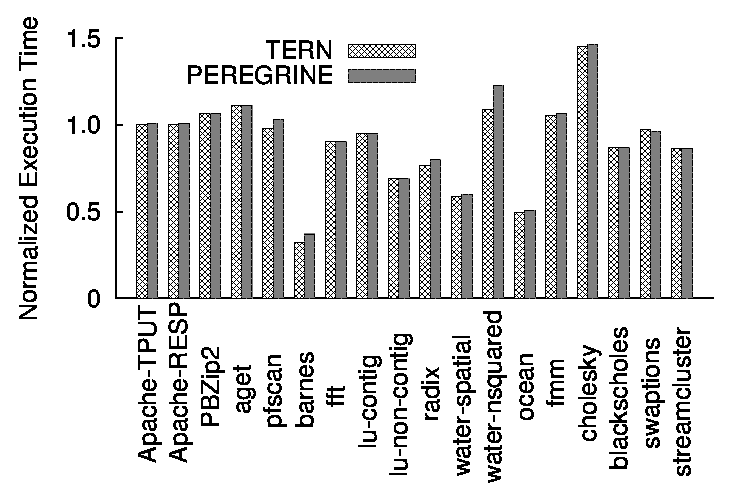
\includegraphics[width=0.5\textwidth]{tern/figures/overhead}

\caption{\small {\em Relative overhead of the replayer over
    nondeterministic execution.} Negative overhead means speedup.}
\label{fig:overhead}
\end{figure}

%% \begin{table}[t]
%% \centering
%% \footnotesize
%% \begin{tabular}{lcc}
%% {\bf Program} &  {\bf Offline} & {\bf Online}\\
%% \hline
%% Apache         &   2.2\%        & \\
%% \pbzip        &   4.96\%       & \\
%% \end{tabular}
%% \caption{\small{\em \tern's online v.s. offline overhead.}}
%% \label{tab:overhead}
%% \end{table}

The most performance-critical component is the replayer because it
operates during the normal execution of a program.
Figure~\ref{fig:overhead} shows the relative overhead of the replayer over
nondeterministic execution, the smaller the better.  For seven out of
the fourteen programs, the replayer performed almost identically to
nondeterministic execution. For \pbzip and barnes, \tern performed
better.  This speedup came partially from the optimization to remove
unnecessary synchronizations, discussed in the next paragraph.  \tern's overhead
for MySQL, volrend, raytrace, water-nsquared, and choleskey is relatively
large because these programs performed many synchronization operations
over a short period of time.  For instance, water-nsquared and cholesky
both call \v{pthread\_mutex\_lock()} and \v{pthread\_mutex\_unlock()} in a
tight loop.

% The replayer's performance degrades with dense synchronization because
% the replayer enforces a total order of the synchronization operations.

%% Although we have not heavily optimized our \tern implementation, it incurs
%% small overhead for nine of the 11 \splash programs. \tern's overhead on
%% water-nsquared and cholesky are higher because they lock and unlock
%% pthread mutexes within a tight loop. However, this overhead is reasonable
%% considering the determinism and stability benefits of \tern.

\begin{figure}[t]
\centering
\includegraphics[width=0.5\textwidth]{tern/figures/opt-overhead}
\caption{\small {\em Overhead reduction by skipping unnecessary
    synchronizations.} ``no opt'' indicates the baseline overhead.}
\label{fig:opt-remove-sync}
\end{figure}

We also measured the effects of skipping unnecessary synchronizations
(\S\ref{sec:skip-waits}).  Figure~\ref{fig:opt-remove-sync} shows the
results.  This optimization significantly reduced the replayer's overhead
for four programs.  Specifically, it made \pbzip and barnes run faster
than nondeterministic execution, and reduced the overhead of
water-nsquared from 172.4\% to 39.1\%.  Its effects on the other programs are
negligible and thus not shown.

\begin{figure}[t]
\centering
\includegraphics[width=0.5\textwidth]{tern/figures/expr-opt-time}
\caption{\small {\em Optimizations to speed up constraint checking.} Note
  the y-axis is broken. ``no opt'' indicates the baseline constraint checking
  time. ``simplify'' refers to the optimization in
  \S\ref{sec:simplify}. ``slice'' refers to the optimization in
  \S\ref{sec:slicing}.}
\label{fig:opt-remove-constraints}
\end{figure}

\begin{table}[t]
\centering
\footnotesize
\begin{tabular}{lcccc}
{\bf Program} &  {\bf Nondet} &  {\bf Memoization} &  {\bf Overhead (times)}\\
\hline
Apache-TPUT   & 462.2 req/s         & 2.1 req/s                &   219.1\\
Apache-RESP   & 0.22 s        & 3.96 s            &   17.0\\
MySQL-TPUT    & 13779.3 req/s      & 172.2 req/s             &   79.0\\
MySQL-RESP    & 0.6 ms       & 61 ms             &   100.6\\
\pbzip        & 0.18 s        & 15.19 s           &   83.4\\
\end{tabular}
\caption{\small{\em Overhead of the memoizer.}}
\label{tab:memoization-overhead}
\end{table}

To reuse a schedule on an input, \tern must check the input against
memoized constraints.  Constraint checking can be costly, and \tern provides
two optimizations to speed it up (\S\ref{sec:simplify} and
\S\ref{sec:slicing}).  Figure~\ref{fig:opt-remove-constraints} shows these
optimizations can effectively speed up constraint checking for Apache,
fft, lu, and radix.  In particular, they reduced the constraint checking
time for lu by 16x.

%% For lu, we have reduced the number of
%% expressions from 145 to 10 by the two mechanisms, and the constraint checking time in replay part has been reduced by 93.8\%, from 7850 us to 492 us. 
%% Branch slicing is more effective than redundancy removal for Apache, redundancy removal is strong than branch slicing in radix.

%% \begin{figure}[t]
%% \centering
%% \includegraphics[width=0.5\textwidth]{figures/memoization-overhead}
%% \vspace{-.1in}
%% \caption{\small {\em Slowdown of the memoizer.}}
%% \vspace{-.2in}
%% \label{fig:memoization-overhead}
%% \end{figure}

Compared to the replayer, the memoizer can run offline, thus its
performance is not as critical.  Table~\ref{tab:memoization-overhead}
shows that this slowdown can sometimes exceed 200x.  The main reason
is that \klee, the symbolic engine used, interprets programs instead of
running them natively.  An instrumentation-based approach can greatly
reduce this slowdown~\cite{cadar:exe:ccs06}, which we plan to implement in
our future work.  
% We did not report the slowdown of the \splash programs because 
% are skewed because the execution time of these programs was too
% short (often 10-100 ms), and \klee's fixed cost of loading a LLVM bitcode
% file dominated the execution time.

% \begin{table*}[t]
% \centering
% \footnotesize
% \begin{tabular}{lccccc}
% {\bf Program} & {\bf no opt} & {\bf w/ simplify} & {\bf w/ slicing} & {\bf w/ both}   \\
% \hline
% fft      &   322.3, 10  & 245.1, 4  & 148.6, 6  & 117.0, 3  \\
% lu      &   7850.4, 145  & 501.1, 13  & 516.8, 16  & 492.0, 10  \\
% radix & 331.5 & 238.0 & 317.6 & 227.9  \\
% Apache &        708.0, 232  & 659.4, 224 & 371.2, 32  & 365.3, 32  \\
% \end{tabular}
% \caption{\small{\em Effects of optimizations of four programs.}}
% \label{tab:overhead}
% \end{table*}

%% Heming: Figure~\ref{fig:overhead} shows the normalized performance of \tern over all the 14 applications, 
%% and six of them (Apache, lu, radix, fmm, ocean, water-spt) have neglible overhead. 
%% \pbzip and barnes have been speed up significantly, since we have removed \v{usleep()} and \v{pthread\_barrier\_wait()} from 
%% them, respectively. This removal is safe and we will discuss it at section X. 
%% Figure~\ref{fig:opt-overhead} shows the speed up after we remove these synchronization operations.
%% In Volrend, the \v{pthread\_barrier\_wait()} operation has also been removed, but it still has a positive overhead (18.5\%).
%% For MySQL, we meaured its overhead and finish rate (shown in Table\ref{tab:stability}) with SysBench simple mode, and the overhead is 69.8\% 
%% (degradation is 30.2\%) and 37.5\% in throughtput and response time. The reason is
%% there are 11.6M synchronization operations within 200,000 sql queries. \tern's overhead is propotional to the number of synchronizations.

%% \begin{figure}[t]
%% \centering
%% \includegraphics[width=0.5\textwidth]{figures/expr-opt-time}
%% \vspace{-.1in}
%% \caption{\small {\em \tern's expression checking time with constraint simplification and slicing.}
%%   Smaller numbers are better}
%% \vspace{-.2in}
%% \label{fig:expr-opt-time}
%% \end{figure}

%% Heming: We have implemented two expression pruning mechanisms
%% in \tern, branching slicing and redundant expression removal. In branch slicing, we use reachability analysis to identify all branches that do not dominate
%% any synchronization operations in source code, and when \tern eliminate all expressions generated from these branchinges. In redundant expression removal,
%% \tern traverse each collected expression with the memoization order and query the STP solver whether this expression is redundant against the other expression, 
%% if so, then it is removed from the expression set. Figure~\ref{fig:expr-opt-time} shows the effects of expression pruning in \tern. For lu, we have reduced the number of
%% expressions from 145 to 10 by the two mechanisms, and the constraint checking time in replay part has been reduced by 93.8\%, from 7850 us to 492 us. 
%% Branch slicing is more effective than redundancy removal for Apache, redundancy removal is strong than branch slicing in radix.


%% % \begin{table*}[t]
%% % \centering
%% % \footnotesize
%% % \begin{tabular}{lcc}
%% % {\bf Program} & {\bf w/ sync} & {\bf w/o syncs} \\
%% % \hline
%% % \pbzip        &   76.5\%   & -8.8\%\\ 
%% % barnes           &   15.4\%    & -18.7\% \\ 
%% % \end{tabular}
%% % \caption{\small{\em Effects of removing synchronization operations.}}
%% % \label{tab:overhead}
%% % \end{table*}

%% \begin{figure}[t]
%% \centering
%% \includegraphics[width=0.5\textwidth]{figures/opt-overhead}
%% \vspace{-.1in}
%% \caption{\small {\em \tern's overhead after removing synchronization operations.}
%%   Smaller numbers are better.}
%% \vspace{-.2in}
%% \label{fig:opt-overhead}
%% \end{figure}

%% \begin{figure}[t]
%% \centering
%% \includegraphics[width=0.5\textwidth]{figures/memoization-overhead}
%% \vspace{-.1in}
%% \caption{\small {\em \tern's memoization overhead for applications.}}
%% \vspace{-.2in}
%% \label{fig:memoization-overhead}
%% \end{figure}

%% We have also investigated the effects of removing synchronization operations in \tern. Since \tern has enforced deterministic order
%% in the \v{before\_landmark()} and \v{after\_landmark()} functions inserted to each synchronization operation, removing synchronization function
%% calls from source code become possible. We have tried to removed \v{usleep()} in the file writer thread from \pbzip and \v{pthread\_barrier\_wait()} from barnes, volrend and water-nsquared,
%% and the speed up is significant. Please note that \v{usleep()} in \pbzip is supposed to reduce contention to acquire pthread mutexes,
%% if we remove them, native exeucutions become more time consuming. Since \tern enforces total order accesses to synchronization objects, it inherently
%% reduces contention, so removing \v{usleep()} can speed up \pbzip. We leave the systermatic investigation of removing synchronization operations in \tern to future work.

%% \subsection{Scalability}

%% \begin{table}[t]
%% \centering
%% \footnotesize
%% \begin{tabular}{lcc}
%% {\bf Program} & {\bf workload} & {\bf Overhead}\\
%% \hline
%% \pbzip        &   &   4.96\%    \\
%% lu            &   &   2.2\%     \\
%% fft           &   &   15.2\%    \\
%% \end{tabular}
%% \caption{\small{\em \tern's overhead.}}
%% \label{tab:overhead}
%% \end{table}


%% \begin{table}[t]
%% \centering
%% \footnotesize
%% \begin{tabular}{lcccc}
%% {\bf Program} & {\bf 8} & {\bf 16} & {\bf 32} & {\bf 64}\\
%% \hline
%% fft           &   6.6\%   &   19.3\%    &   32.6\%   &   4.7\%     \\
%% lu           &   3.8\%   &   3.2\%    &   -0.2\%   &   8.4\%     \\
%% barnes           &   4.8\%   &   13.4\%    &   44.6\%   &   135.8\%     \\
%% radix           &   12.2\%   &   41.8\%    &   85.9\%   &   94.8\%     \\
%% fmm           &   25.9\%   &   22.9\%    &   29.3\%   &   36.6\%     \\
%% ocean           &   x\%   &   x\%    &   x\%   &   x\%     \\
%% volrend           &   x\%   &   x\%    &   x\%   &   x\%     \\
%% water-spatial           &   64.0\%   &   69.5\%    &   74.9\%   &   101.9\%     \\
%% raytrace           &   204.7\%   &   319.8\%    &   281.3\%   &   152.3\%     \\
%% water-nsquared           &   x\%   &   x\%    &   x\%   &   x\%     \\
%% cholesky           &   195.7\%   &   501.0\%    &   114.02\%   &   N/A\%     \\
%% \end{tabular}
%% \caption{\small{\em \tern's overhead in scalability.}}
%% \label{tab:overhead-scalability}
%% \end{table}


\subsection{Determinism}\label{sec:determinism}

We evaluated \tern's determinism via three sets of experiments.  The first
set checked the memoized schedules for races (\S\ref{sec:race-results}).
The second evaluated \tern's ability to deterministically reproduce or avoid
bugs (\S\ref{sec:bug-determinism}).  The third measured how deterministic
memory accesses are with and without
\tern (\S\ref{sec:memory-determinism}).

\subsubsection{Race Detection Results}\label{sec:race-results}

When memoizing schedules for each of the 14 programs, we turned on \tern's
race detector.  We found that except for radix and cholesky, the schedules
\tern memoized for all other programs were free of schedule races and
symbolic races with respect to the symbolic data we annotated
(\S\ref{sec:detect-race}).  Our race detection result is not surprising
because most schedules are indeed race free.  It implies that, for runs
that reuse the memoized schedules of all programs but radix and cholesky,
\tern ensures determinism, barring the assumption discussed in
\S\ref{sec:detect-race}.

\subsubsection{Bug Determinism}\label{sec:bug-determinism}

%\hspace{-.1in}
\begin{table}[t]
\begin{center}
{
\small
\begin{tabular}{lp{2.3in}}

{\bf Program} & {\bf Error Description} \\

\hline

Apache & Reference count decrement and check against 0 are not atomic.\\

\pbzip & Variable \v{fifo} is used in one thread after being freed by another.\\


% Mozilla-73761 & Accessing the property cache array and its flag are not
% atomic.  \\

% Mozilla-201134 & Accumulative updates to a security flag called
% \v{nsCertType} are atomic. \\

% Mozilla-133773 & A hash table in a global variable called
% \v{atomState} is used after 
fft & \v{initdonetime} and  \v{finishtime} are read
before assigned the correct values.\\

lu & Variable \v{rf} is read before assigned the  correct
value. \\

barnes & Variable \v{tracktime} is read before assigned the
correct value.\\

\end{tabular}}
\end{center}
\caption{{\em Concurrency errors used in evaluation}.} \label{table:races}
\end{table}

We also evaluated how deterministically \tern could reproduce or avoid
bugs.  Table~\ref{table:races} lists five real concurrency bugs we used.
We selected them because they were frequently used in previous
studies~\cite{avio:asplos06,ctrigger:asplos09,lu:concurrency-bugs,pres:sosp09}
and we could reproduce them on our evaluation machine.  To measure bug
determinism, we first memoized schedules for programs listed in
Table~\ref{table:races}.  We then manually inserted \v{usleep()} to these
programs to get alternate schedules.  We then ran the buggy programs
again, reusing the memoized schedules.  We also injected random delays
into the reuse runs to perturb timing.  We found that, \tern consistently
reproduced or avoided all five bugs.  We verified this result
by inspecting the memoized schedules.

\subsubsection{Memory Access Determinism}\label{sec:memory-determinism}

\tern enforces synchronization orders, which should make memory access
orders more deterministic.  We quantified this effect over Apache and
\pbzip.  Specifically, we instrumented Apache with LLVM to trace accesses
to global variables and the heap, a crude approximation of shared memory.
We ran Apache with \tern to serve five HTTP requests and collected a trace
of memory accesses.  We then repeated this experiment 20 times to collect
20 traces, and computed the average pairwise edit
distance~\cite{edit-distance}.  We then measured the same edit distance
for Apache in nondeterministic execution mode and compared the two.  We
did the same comparison for \pbzip with a decompression workload of 2MB.  
Table~\ref{tab:memory-determinism} shows the result.  For Apache,
runs with \tern were 7.97 times more deterministic than those without.  For
\pbzip, \tern was 2.33 times more deterministic, but the memory trace had
only 1,234 accesses on average.


\begin{table}
\centering
\small
\begin{tabular}{ccccc}
{\bf Program} & {\bf Length} & {\bf Nondet} & {\tern} & {\bf Ratio} \\
\hline
Apache & 148,058 & 86,215 & 10,821 & 7.97 \\
\pbzip & 1,234   & 161   & 69    & 2.33 \\
\end{tabular}
\caption{\small{\em Memory access determinism.}  We traced memory accessed
  only from \pbzip, not the external BZip2
  library.} \label{tab:memory-determinism}
\end{table}


%%  serve five concurrent requests and memoize a
%% memory access trace.  We then repeated 20 times to collect 20 traces.  We
%% then computed the pairwise edit distances~\cite{edit-distance} of the
%% traces and take the average.  We then did the same set of experiments for
%% Apache with \tern and compared the average edit distances of the two.  We
%% did the same set of experiments for \pbzip with a decompression workload
%% of a 2MB file.  Table~\ref{tab:memory-determinism} shows the result.  For
%% Apache, executions with \tern are 7.97 times more deterministic than
%% executions without.  For \pbzip, \tern is only 2.33 times more
%% deterministic, but the memory trace contains only 1,234 accesses on
%% average.




%% As discussed in \S\ref{sec:define-schedule}, \tern aims to enforce a
%% deterministic synchronization order.  This order should make memory
%% accesses highly deterministic as well.  In this section, we quantified
%% memory access determinism on server program Apache and batch program
%% \pbzip.

%% \begin{table}
%% \centering
%% \small
%% \begin{tabular}{ccccc}
%% {\bf Program} & {\bf Len} & {\bf W/o \tern} & {\bf W/ \tern} & {\bf Ratio} \\
%% \hline
%% Apache & 148,058 & 86,215 & 10,821 & 7.97 \\
%% \pbzip & 1,234   & 161   & 69    & 2.33 \\
%% \end{tabular}
%% \caption{\small{\em Memory access determinism results.} Column {\bf Len}
%%   shows the lengths of the memory traces.  {\bf W/o \tern} shows the average
%%   edit distance for executions without \tern.  {\bf W/ \tern} shows the
%%   average edit distance with \tern.  {\bf Ratio} reports the ratio between
%%   the two edit distances.  \tern makes Apache 7.97 times more
%%   deterministic, but only 2.33 times for \pbzip, because \pbzip only
%%   accessed fewer than 140 distinct memory locations. Note we only trace
%%   memory accessed made by \pbzip, not the external BZip2
%%   library.} \label{tab:memory-determinism}
%% \end{table}

%% We instrumented Apache with LLVM to trace accesses to global variables and
%% the heap, a crude approximation of shared memory.  We ran Apache without
%% \tern to serve five concurrent requests and memoize a memory access trace.
%% We then repeated 20 times to collect 20 traces.  We then computed the
%% pairwise edit distances~\cite{edit-distance} of the traces and take the
%% average.  We then did the same set of experiments for Apache with \tern and
%% compared the average edit distances of the two.  We did the same set of
%% experiments for \pbzip with a decompression workload of a 2MB file.
%% Table~\ref{tab:memory-determinism} shows the result.  For Apache,
%% executions with \tern are 7.97 times more deterministic than executions
%% without.  For \pbzip, \tern is only 2.33 times more deterministic, but the
%% memory trace contains only 1,234 accesses on average.

%% \begin{figure}[t]
%%   \centering
%% % YJF: commented them out so build of the paper is faster.  
%% %  \includegraphics[width=2.5in]{figures/determinism/httpd-window/httpd-order-window-merge-10.eps}
%% %  \includegraphics[width=2.5in]{figures/determinism/httpd-window/httpd-order-window-merge-20.eps}
%% %  \includegraphics[width=2.5in]{figures/determinism/httpd-window/httpd-no-order-window-merge-10.eps}
%% %  \includegraphics[width=2.5in]{figures/determinism/httpd-window/httpd-no-order-window-merge-20.eps}
%%   \caption{{\em Memory accesses collected from the memory determinism
%%       experiments.}}
%% \label{fig:memory-determinism}
%% \end{figure}


%% Figure~\ref{fig:memory-determinism} shows the memory accesses collected
%% from this set of four experiments.  

%% For each experiment, we overlay all
%% memory accesses from 20 runs in one subfigure, which each access maps to a
%% point.  We assign a unique ID to each memory address traced to neutralize
%% address space layout randomization~\cite{aslr}.  The more deterministic
%% the memory accesses, the more empty space is in the subfigures because
%% points are placed on top of other points.  As shown in the subfigures,
%% runs with \tern are more deterministic than runs without.


%% evaluate the bug repeatability of \tern.  For \pbzip, the default
%% schedule \tern selects exposes the error.  For each of the other errors, we
%% have to manually insert 2-4 \v{sleep(0)} calls in the corresponding
%% program to expose the error.  We let \tern memoize these buggy schedules.
%% We then remove the bogus \v{sleep(0)} calls we insert from the programs.
%% We also remove the \v{before\_blocking()} and \v{after\_blocking()} calls
%% due to the bogus \v{sleep(0)} calls from the memoized schedules.  We rerun
%% the programs with the memoized schedules and observe that the bugs can
%% always be reproduced.  

%% manually injected yields

%% apache: 4
%% pbzip2: 0.  always show up.  race always occur.  order determined.  
%% lu: 3       
%% barnes: 3
%% fft: 2

% manually inspect the log and ensure that original bug masked by the total
% order of sync memoized.

% more stuff.  list the bugs.  say specifically how experiments are done.





% micro benchmarks.  constraint checking time.

%% \begin{figure}[t]
%%   \centering
%%   \caption{{\em \tern's scalability.}}
%% \label{fig:scalability}
%% \end{figure}

%% We also measure \tern's scalability by varying the number of threads.
%% Figure~\ref{fig:scalability} shows the results on XX and XX.  \tern scales
%% well as the number of threads increases.  Indeed, XXX highlight.


%% The most important thing is to verify whether the instrumented x86 programs running with my constraints and thread ids total 
%% order hurt performance, including response time and throughtput. Overhead less than 10\% is nice.

%% Another metric professor has mentioned before is this graph: as the number of constraints we have collected grow up,
%% does the curve of the coverage increase as a log() curve?

%% Note: how deterministic improvement after \tern is applied.

%% Note: how fast to collect constraints in klee? Is klee interpreter too slow to be used as a shadow program? That is, let klee run parallelly as a shadow program with 
%% the x86 exe file, when an input comes, duplicate the input and send each of them to exe file and klee, so while the exe file is running,
%% klee can collect constraints on the way.

%% Three main metrics in evaluation:

%% 1 overhead (execution time, response time, throughput);

%% 2 how deterministic (compre one by one seed, C(m,n));

%% Note: we measure the load and store instructions to shared memory as the determinism metric, and memory 
%% addresses are normalized. CTrigger uses the number of "unserializable interleavings" in Figure 4 and 5 in their paper to 
%% measure "similarity between runs". Actually our results are not conflict to theirs: even most of executions exercise most of 
%% the same buggy interleavings, that does not mean memory references in different runs are the mostly the same.

%% Essentially, our work focuses on deterministic execution (not only hiding or exposing bugs, but also producing the same 
%% output for the same input, so actually our goals are more than CTrigger's goals), and determinism of memory references are 
%% the main concern of our approach, so we use this metric. 


%% 3 how reliable to expose or hide bugs;

%% 4 coverage (randomly select some input, check the curve);

%\begin{figure*}[t]
%  \centering
% YJF: commented them out so build of the paper is faster.  
%  \includegraphics[width=2.5in]{figures/determinism/httpd-window/httpd-order-window-merge-10.eps}
%  \includegraphics[width=2.5in]{figures/determinism/httpd-window/httpd-order-window-merge-20.eps}
%  \includegraphics[width=2.5in]{figures/determinism/httpd-window/httpd-no-order-window-merge-10.eps}
%  \includegraphics[width=2.5in]{figures/determinism/httpd-window/httpd-no-order-window-merge-20.eps}
%  \caption{Execution determinism in Apache}
%\label{fig:determinism-httpd-window}
%\end{figure*}

%% \begin{table*}[t]
%% \centering
%% \footnotesize
%% \begin{tabular}{lc}
%% {\bf Program} & {\bf Number of Race detected}\\
%% \hline
%% radix           &   1\\ 
%% cholesky        &   1\\ 
%% \end{tabular}
%% \caption{\small{\em Races detected in all programs.}}
%% \label{tab:races}
%% \end{table*}

%% \begin{table*}[t]
%% \centering
%% \footnotesize
%% \begin{tabular}{lc}
%% {\bf Program} & {\bf Number of wild order constraints}\\
%% \hline
%% fmm        &   1\\
%% volrend        &   1\\
%% cholesky       &   1\\
%% \end{tabular}
%% \caption{\small{\em Wild order constraints in all programs.}}
%% \label{tab:wild-order}
%% \end{table*}




